\begin{figure}
    \centering
    \tikzset{every picture/.style={line width=0.75pt}} %set default line width to 0.75pt        
    \caption{\label{fig:M1}As áreas do conhecimento linguístico} 
    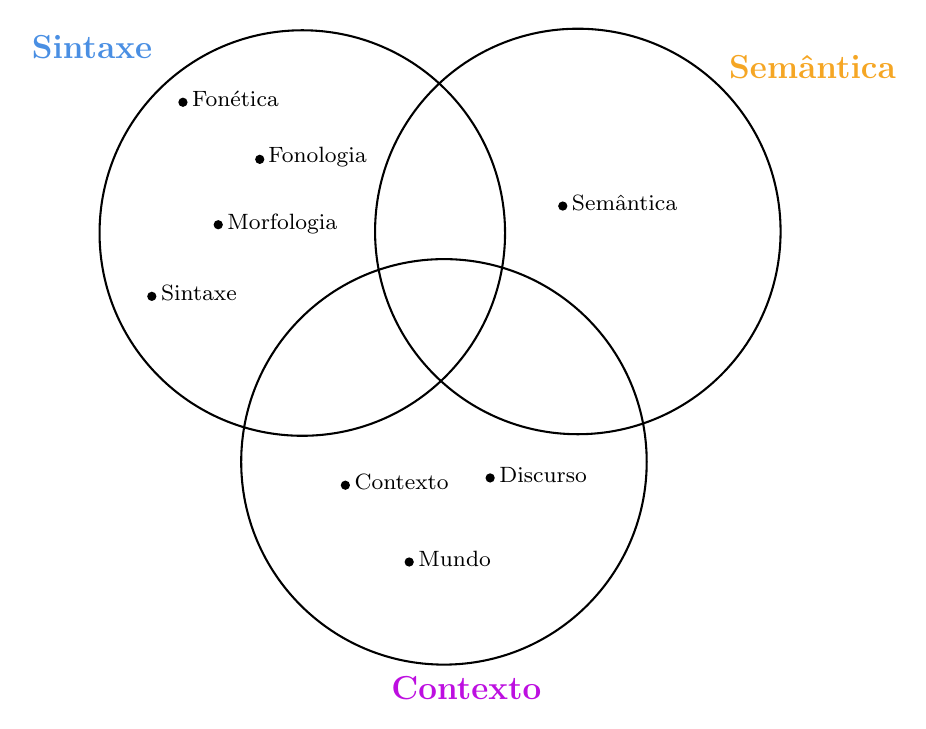
\begin{tikzpicture}[x=0.75pt,y=0.75pt,yscale=-0.75,xscale=0.75]
    %uncomment if require: \path (0,519); %set diagram left start at 0, and has height of 519
    
    %Shape: Circle [id:dp6775411490734827] 
    \draw   (75.5,169.25) .. controls (75.5,97.31) and (133.81,39) .. (205.75,39) .. controls (277.69,39) and (336,97.31) .. (336,169.25) .. controls (336,241.19) and (277.69,299.5) .. (205.75,299.5) .. controls (133.81,299.5) and (75.5,241.19) .. (75.5,169.25) -- cycle ;
    %Shape: Circle [id:dp7013179161415731] 
    \draw   (252.5,168.25) .. controls (252.5,96.31) and (310.81,38) .. (382.75,38) .. controls (454.69,38) and (513,96.31) .. (513,168.25) .. controls (513,240.19) and (454.69,298.5) .. (382.75,298.5) .. controls (310.81,298.5) and (252.5,240.19) .. (252.5,168.25) -- cycle ;
    %Shape: Circle [id:dp9236852908414266] 
    \draw   (166.5,316.25) .. controls (166.5,244.31) and (224.81,186) .. (296.75,186) .. controls (368.69,186) and (427,244.31) .. (427,316.25) .. controls (427,388.19) and (368.69,446.5) .. (296.75,446.5) .. controls (224.81,446.5) and (166.5,388.19) .. (166.5,316.25) -- cycle ;
    %Shape: Circle [id:dp8411900099296108] 
    \draw  [color={rgb, 255:red, 0; green, 0; blue, 0 }  ,draw opacity=1 ][fill={rgb, 255:red, 0; green, 0; blue, 0 }  ,fill opacity=1 ] (126.83,85.25) .. controls (126.83,84.01) and (127.84,83) .. (129.08,83) .. controls (130.33,83) and (131.33,84.01) .. (131.33,85.25) .. controls (131.33,86.49) and (130.33,87.5) .. (129.08,87.5) .. controls (127.84,87.5) and (126.83,86.49) .. (126.83,85.25) -- cycle ;
    
    %Shape: Circle [id:dp42285790681396784] 
    \draw  [color={rgb, 255:red, 0; green, 0; blue, 0 }  ,draw opacity=1 ][fill={rgb, 255:red, 0; green, 0; blue, 0 }  ,fill opacity=1 ] (176.17,121.92) .. controls (176.17,120.67) and (177.17,119.67) .. (178.42,119.67) .. controls (179.66,119.67) and (180.67,120.67) .. (180.67,121.92) .. controls (180.67,123.16) and (179.66,124.17) .. (178.42,124.17) .. controls (177.17,124.17) and (176.17,123.16) .. (176.17,121.92) -- cycle ;
    %Shape: Circle [id:dp5438038252660116] 
    \draw  [color={rgb, 255:red, 0; green, 0; blue, 0 }  ,draw opacity=1 ][fill={rgb, 255:red, 0; green, 0; blue, 0 }  ,fill opacity=1 ] (149.5,163.92) .. controls (149.5,162.67) and (150.51,161.67) .. (151.75,161.67) .. controls (152.99,161.67) and (154,162.67) .. (154,163.92) .. controls (154,165.16) and (152.99,166.17) .. (151.75,166.17) .. controls (150.51,166.17) and (149.5,165.16) .. (149.5,163.92) -- cycle ;
    
    %Shape: Circle [id:dp7047187084507844] 
    \draw  [color={rgb, 255:red, 0; green, 0; blue, 0 }  ,draw opacity=1 ][fill={rgb, 255:red, 0; green, 0; blue, 0 }  ,fill opacity=1 ] (106.83,209.92) .. controls (106.83,208.67) and (107.84,207.67) .. (109.08,207.67) .. controls (110.33,207.67) and (111.33,208.67) .. (111.33,209.92) .. controls (111.33,211.16) and (110.33,212.17) .. (109.08,212.17) .. controls (107.84,212.17) and (106.83,211.16) .. (106.83,209.92) -- cycle ;
    
    %Shape: Circle [id:dp2978376246917125] 
    \draw  [color={rgb, 255:red, 0; green, 0; blue, 0 }  ,draw opacity=1 ][fill={rgb, 255:red, 0; green, 0; blue, 0 }  ,fill opacity=1 ] (370.83,151.92) .. controls (370.83,150.67) and (371.84,149.67) .. (373.08,149.67) .. controls (374.33,149.67) and (375.33,150.67) .. (375.33,151.92) .. controls (375.33,153.16) and (374.33,154.17) .. (373.08,154.17) .. controls (371.84,154.17) and (370.83,153.16) .. (370.83,151.92) -- cycle ;
    
    %Shape: Circle [id:dp5234260157724945] 
    \draw  [color={rgb, 255:red, 0; green, 0; blue, 0 }  ,draw opacity=1 ][fill={rgb, 255:red, 0; green, 0; blue, 0 }  ,fill opacity=1 ] (231.17,331.25) .. controls (231.17,330.01) and (232.17,329) .. (233.42,329) .. controls (234.66,329) and (235.67,330.01) .. (235.67,331.25) .. controls (235.67,332.49) and (234.66,333.5) .. (233.42,333.5) .. controls (232.17,333.5) and (231.17,332.49) .. (231.17,331.25) -- cycle ;
    
    %Shape: Circle [id:dp004866918106716023] 
    \draw  [color={rgb, 255:red, 0; green, 0; blue, 0 }  ,draw opacity=1 ][fill={rgb, 255:red, 0; green, 0; blue, 0 }  ,fill opacity=1 ] (324.17,326.58) .. controls (324.17,325.34) and (325.17,324.33) .. (326.42,324.33) .. controls (327.66,324.33) and (328.67,325.34) .. (328.67,326.58) .. controls (328.67,327.83) and (327.66,328.83) .. (326.42,328.83) .. controls (325.17,328.83) and (324.17,327.83) .. (324.17,326.58) -- cycle ;
    
    %Shape: Circle [id:dp8947660528209017] 
    \draw  [color={rgb, 255:red, 0; green, 0; blue, 0 }  ,draw opacity=1 ][fill={rgb, 255:red, 0; green, 0; blue, 0 }  ,fill opacity=1 ] (272.17,380.58) .. controls (272.17,379.34) and (273.17,378.33) .. (274.42,378.33) .. controls (275.66,378.33) and (276.67,379.34) .. (276.67,380.58) .. controls (276.67,381.83) and (275.66,382.83) .. (274.42,382.83) .. controls (273.17,382.83) and (272.17,381.83) .. (272.17,380.58) -- cycle ;
    
    % Text Node
    \draw (182,112) node [anchor=north west][inner sep=0.75pt]   [align=left] {{\footnotesize Fonologia}};
    % Text Node
    \draw (133,76.33) node [anchor=north west][inner sep=0.75pt]   [align=left] {{\footnotesize Fonética}};
    % Text Node
    \draw (155.67,155) node [anchor=north west][inner sep=0.75pt]   [align=left] {{\footnotesize Morfologia}};
    % Text Node
    \draw (113,201) node [anchor=north west][inner sep=0.75pt]   [align=left] {{\footnotesize Sintaxe}};
    % Text Node
    \draw (377,143) node [anchor=north west][inner sep=0.75pt]   [align=left] {{\footnotesize Semântica}};
    % Text Node
    \draw (237.33,322.33) node [anchor=north west][inner sep=0.75pt]   [align=left] {{\footnotesize Contexto}};
    % Text Node
    \draw (330.33,317.67) node [anchor=north west][inner sep=0.75pt]   [align=left] {{\footnotesize Discurso}};
    % Text Node
    \draw (278.33,371.67) node [anchor=north west][inner sep=0.75pt]   [align=left] {{\footnotesize Mundo}};
    % Text Node
    \draw (30,40) node [anchor=north west][inner sep=0.75pt]   [align=left] {{\large \textbf{\textcolor[rgb]{0.29,0.56,0.89}{Sintaxe}}}};
    % Text Node
    \draw (478,53) node [anchor=north west][inner sep=0.75pt]   [align=left] {{\large \textbf{\textcolor[rgb]{0.96,0.65,0.14}{Semântica}}}};
    % Text Node
    \draw (261,452) node [anchor=north west][inner sep=0.75pt]   [align=left] {{\large \textbf{\textcolor[rgb]{0.74,0.06,0.88}{Contexto}}}};
    \end{tikzpicture}
    \fonte{Do autor\footnotemark}
\end{figure}

\footnotetext{Elaborada conforme sugerido por \citeonline{allen1988natural} e \citeonline{cambria2014jumping}}